\documentclass[a4paper]{book}
\usepackage{makeidx}
\usepackage{natbib}
\usepackage{graphicx}
\usepackage{multicol}
\usepackage{float}
\usepackage{listings}
\usepackage{color}
\usepackage{ifthen}
\usepackage[table]{xcolor}
\usepackage{textcomp}
\usepackage{alltt}
\usepackage{ifpdf}
\ifpdf
\usepackage[pdftex,
            pagebackref=true,
            colorlinks=true,
            linkcolor=blue,
            unicode
           ]{hyperref}
\else
\usepackage[ps2pdf,
            pagebackref=true,
            colorlinks=true,
            linkcolor=blue,
            unicode
           ]{hyperref}
\usepackage{pspicture}
\fi
\usepackage[utf8]{inputenc}
\usepackage{polski}
\usepackage[T1]{fontenc}

\usepackage{mathptmx}
\usepackage[scaled=.90]{helvet}
\usepackage{courier}
\usepackage{sectsty}
\usepackage[titles]{tocloft}
\usepackage{doxygen}
\lstset{language=C++,inputencoding=utf8,basicstyle=\footnotesize,breaklines=true,breakatwhitespace=true,tabsize=8,numbers=left }
\makeindex
\setcounter{tocdepth}{3}
\renewcommand{\footrulewidth}{0.4pt}
\renewcommand{\familydefault}{\sfdefault}
\hfuzz=15pt
\setlength{\emergencystretch}{15pt}
\hbadness=750
\tolerance=750
\begin{document}
\hypersetup{pageanchor=false,citecolor=blue}
\begin{titlepage}
\vspace*{7cm}
\begin{center}
{\Large \-Lab4 }\\
\vspace*{1cm}
{\large \-Wygenerowano przez Doxygen 1.7.6.1}\\
\vspace*{0.5cm}
{\small Sun Mar 30 2014 22:58:16}\\
\end{center}
\end{titlepage}
\clearemptydoublepage
\pagenumbering{roman}
\tableofcontents
\clearemptydoublepage
\pagenumbering{arabic}
\hypersetup{pageanchor=true,citecolor=blue}
\chapter{\-Dokumentacja zadania \-P\-A\-M\-S\-I \-L\-A\-B 4}
\label{index}\hypertarget{index}{}\begin{DoxyAuthor}{\-Autor}
\-Martyna \-Bandura 
\end{DoxyAuthor}
\begin{DoxyDate}{\-Data}
19.\-03.\-2014 
\end{DoxyDate}

\chapter{\-Struktura katalogów}
\section{\-Katalogi}
\-Ta struktura katalogów jest posortowana jest z grubsza, choć nie całkowicie, alfabetycznie\-:\begin{DoxyCompactList}
\item \contentsline{section}{prj}{\pageref{dir_9f92f53661fd78c561fa1672d6c740cd}}{}
\end{DoxyCompactList}

\chapter{\-Indeks klas}
\section{\-Lista klas}
\-Tutaj znajdują się klasy, struktury, unie i interfejsy wraz z ich krótkimi opisami\-:\begin{DoxyCompactList}
\item\contentsline{section}{\hyperlink{class_drzewo}{\-Drzewo$<$ K, W $>$} \\*\-Modeluje pojecie drzewa binarnego. \-Jego atrybutem jest klasa \hyperlink{class_wezel}{\-Wezel} }{\pageref{class_drzewo}}{}
\item\contentsline{section}{\hyperlink{class_para}{\-Para$<$ K, W $>$} \\*\-Modeluje pojecie pary. \-Jej atrybutem sa pola zawierajace klucz i wartosci }{\pageref{class_para}}{}
\item\contentsline{section}{\hyperlink{class_tablica}{\-Tablica$<$ K, W $>$} \\*\-Modeluje pojecie tablicy z haszowaniem. \-Klasa modeluje pojecie tablicy z haszowaniem. \-Jej atrybutami sa pola\-: klucz i wartosc }{\pageref{class_tablica}}{}
\item\contentsline{section}{\hyperlink{class_wezel}{\-Wezel$<$ K, W $>$} \\*\-Modeluje pojecie wezla. \-Jego atrybutem jest klasa \hyperlink{class_para}{\-Para} }{\pageref{class_wezel}}{}
\end{DoxyCompactList}

\chapter{\-Indeks plików}
\section{\-Lista plików}
\-Tutaj znajduje się lista wszystkich plików z ich krótkimi opisami\-:\begin{DoxyCompactList}
\item\contentsline{section}{\hyperlink{main_8cpp}{main.\-cpp} \\*\-Plik zawiera glowna funkcje programu }{\pageref{main_8cpp}}{}
\item\contentsline{section}{\hyperlink{simplex_8cpp}{simplex.\-cpp} \\*\-Definicje poszczegolnych funkcji dla klasy \hyperlink{class_simplex}{\-Simplex} }{\pageref{simplex_8cpp}}{}
\item\contentsline{section}{\hyperlink{simplex_8h}{simplex.\-h} \\*\-Plik naglowkowy klasy \hyperlink{class_simplex}{\-Simplex} }{\pageref{simplex_8h}}{}
\end{DoxyCompactList}

\chapter{\-Dokumentacja katalogów}
\hypertarget{dir_c07a9c7beb5be1f9263fa9a4a27d497a}{\section{\-Dokumentacja katalogu inc/}
\label{dir_c07a9c7beb5be1f9263fa9a4a27d497a}\index{\-Dokumentacja katalogu inc/@{\-Dokumentacja katalogu inc/}}
}
\-Directory dependency graph for inc/\-:\nopagebreak
\begin{figure}[H]
\begin{center}
\leavevmode
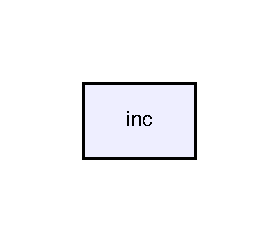
\includegraphics[width=134pt]{dir_c07a9c7beb5be1f9263fa9a4a27d497a_dep}
\end{center}
\end{figure}
\subsection*{\-Pliki}
\begin{DoxyCompactItemize}
\item 
plik \hyperlink{dzialania_8hpp}{dzialania.\-hpp}
\item 
plik \hyperlink{merge_8hpp}{merge.\-hpp}
\item 
plik \hyperlink{quick_8hpp}{quick.\-hpp}
\item 
plik \hyperlink{tablica_8hpp}{tablica.\-hpp}
\end{DoxyCompactItemize}

\hypertarget{dir_40848eaed652bede2b8acd305f90d5c5}{\section{\-Dokumentacja katalogu src/}
\label{dir_40848eaed652bede2b8acd305f90d5c5}\index{\-Dokumentacja katalogu src/@{\-Dokumentacja katalogu src/}}
}
\-Directory dependency graph for src/\-:\nopagebreak
\begin{figure}[H]
\begin{center}
\leavevmode
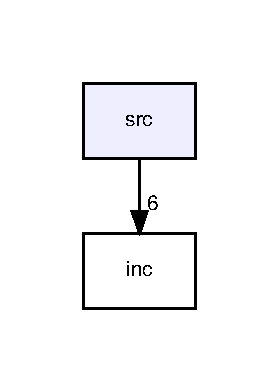
\includegraphics[width=134pt]{dir_40848eaed652bede2b8acd305f90d5c5_dep}
\end{center}
\end{figure}
\subsection*{\-Pliki}
\begin{DoxyCompactItemize}
\item 
plik \hyperlink{dzialania_8cpp}{dzialania.\-cpp}
\item 
plik \hyperlink{glowny_8cpp}{glowny.\-cpp}
\item 
plik \hyperlink{merge_8cpp}{merge.\-cpp}
\item 
plik \hyperlink{quick_8cpp}{quick.\-cpp}
\item 
plik \hyperlink{tablica_8cpp}{tablica.\-cpp}
\end{DoxyCompactItemize}

\chapter{\-Dokumentacja klas}
\hypertarget{class_dzialania}{\section{\-Dokumentacja klasy \-Dzialania}
\label{class_dzialania}\index{\-Dzialania@{\-Dzialania}}
}


{\ttfamily \#include $<$dzialania.\-hpp$>$}



\-Diagram współpracy dla \-Dzialania\-:\nopagebreak
\begin{figure}[H]
\begin{center}
\leavevmode
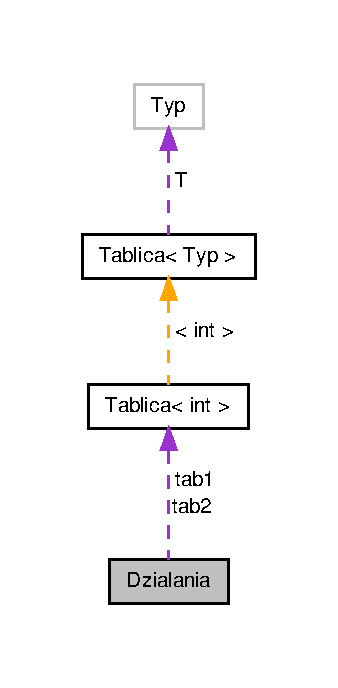
\includegraphics[width=162pt]{class_dzialania__coll__graph}
\end{center}
\end{figure}
\subsection*{\-Metody publiczne}
\begin{DoxyCompactItemize}
\item 
bool \hyperlink{class_dzialania_a4d1a1b41a0f2f76d4c16ad20f77b7cfa}{wczytajplik} (char $\ast$nazwapl)
\item 
bool \hyperlink{class_dzialania_af059b80e034854eb1ae878d6b636fff6}{porownaj} (char $\ast$nazwapl)
\item 
int \hyperlink{class_dzialania_a177e69d16b8280aae1d658adb67a8fbc}{rozmiartab} ()
\item 
double \hyperlink{class_dzialania_a8c13fb89281d74f9dd8dd22f43bffbb9}{liczczas} (int iloscpowtorzen)
\end{DoxyCompactItemize}
\subsection*{\-Metody prywatne}
\begin{DoxyCompactItemize}
\item 
void \hyperlink{class_dzialania_a5e82b0cea1d28ce02b6968071c1d20e5}{oblicz} ()
\end{DoxyCompactItemize}
\subsection*{\-Atrybuty prywatne}
\begin{DoxyCompactItemize}
\item 
\hyperlink{class_tablica}{\-Tablica}$<$ int $>$ \hyperlink{class_dzialania_ab4b7bdba95ea206363cf4d0366bf0be5}{tab1}
\item 
\hyperlink{class_tablica}{\-Tablica}$<$ int $>$ \hyperlink{class_dzialania_ac226e6f7c3854fb9ed36dec2ff476399}{tab2}
\end{DoxyCompactItemize}


\subsection{\-Opis szczegółowy}
\-Deklaracja klasy \hyperlink{class_dzialania}{\-Dzialania}. 

\-Klasa \hyperlink{class_dzialania}{\-Dzialania} posiada funkcje potrzebne do wykonywania dzialan na tablicach . 

\subsection{\-Dokumentacja funkcji składowych}
\hypertarget{class_dzialania_a8c13fb89281d74f9dd8dd22f43bffbb9}{\index{\-Dzialania@{\-Dzialania}!liczczas@{liczczas}}
\index{liczczas@{liczczas}!Dzialania@{\-Dzialania}}
\subsubsection[{liczczas}]{\setlength{\rightskip}{0pt plus 5cm}double {\bf \-Dzialania\-::liczczas} (
\begin{DoxyParamCaption}
\item[{int}]{iloscpowtorzen}
\end{DoxyParamCaption}
)}}\label{class_dzialania_a8c13fb89281d74f9dd8dd22f43bffbb9}
liczczas -\/ zmienna zawiera ile powtorzen ma wykonac program \hypertarget{class_dzialania_a5e82b0cea1d28ce02b6968071c1d20e5}{\index{\-Dzialania@{\-Dzialania}!oblicz@{oblicz}}
\index{oblicz@{oblicz}!Dzialania@{\-Dzialania}}
\subsubsection[{oblicz}]{\setlength{\rightskip}{0pt plus 5cm}void {\bf \-Dzialania\-::oblicz} (
\begin{DoxyParamCaption}
{}
\end{DoxyParamCaption}
)\hspace{0.3cm}{\ttfamily  \mbox{[}private\mbox{]}}}}\label{class_dzialania_a5e82b0cea1d28ce02b6968071c1d20e5}


\-Funkcja wykonujaca dzialanie mnozenia danych z pliku 2 razy. 

\-Najwazniejsze pola funkcji \hypertarget{class_dzialania_af059b80e034854eb1ae878d6b636fff6}{\index{\-Dzialania@{\-Dzialania}!porownaj@{porownaj}}
\index{porownaj@{porownaj}!Dzialania@{\-Dzialania}}
\subsubsection[{porownaj}]{\setlength{\rightskip}{0pt plus 5cm}bool {\bf \-Dzialania\-::porownaj} (
\begin{DoxyParamCaption}
\item[{char $\ast$}]{nazwapl}
\end{DoxyParamCaption}
)}}\label{class_dzialania_af059b80e034854eb1ae878d6b636fff6}
\-Funkcja porownuje dwa pliki \-: plik wejsciowy i sprawdzajacy. \hypertarget{class_dzialania_a177e69d16b8280aae1d658adb67a8fbc}{\index{\-Dzialania@{\-Dzialania}!rozmiartab@{rozmiartab}}
\index{rozmiartab@{rozmiartab}!Dzialania@{\-Dzialania}}
\subsubsection[{rozmiartab}]{\setlength{\rightskip}{0pt plus 5cm}int {\bf \-Dzialania\-::rozmiartab} (
\begin{DoxyParamCaption}
{}
\end{DoxyParamCaption}
)\hspace{0.3cm}{\ttfamily  \mbox{[}inline\mbox{]}}}}\label{class_dzialania_a177e69d16b8280aae1d658adb67a8fbc}
\-Funkcja mierzy czas działania

/$\ast$! \-Funkcja zwraca rozmiar danej tablicy. \hypertarget{class_dzialania_a4d1a1b41a0f2f76d4c16ad20f77b7cfa}{\index{\-Dzialania@{\-Dzialania}!wczytajplik@{wczytajplik}}
\index{wczytajplik@{wczytajplik}!Dzialania@{\-Dzialania}}
\subsubsection[{wczytajplik}]{\setlength{\rightskip}{0pt plus 5cm}bool {\bf \-Dzialania\-::wczytajplik} (
\begin{DoxyParamCaption}
\item[{char $\ast$}]{nazwapl}
\end{DoxyParamCaption}
)}}\label{class_dzialania_a4d1a1b41a0f2f76d4c16ad20f77b7cfa}
\-Funkcja wczytujaca plik. \-Sprawdza także poprawność wykonania operacji.

nazwapl zmienna zawierajaca nazwe pliku 

\subsection{\-Dokumentacja atrybutów składowych}
\hypertarget{class_dzialania_ab4b7bdba95ea206363cf4d0366bf0be5}{\index{\-Dzialania@{\-Dzialania}!tab1@{tab1}}
\index{tab1@{tab1}!Dzialania@{\-Dzialania}}
\subsubsection[{tab1}]{\setlength{\rightskip}{0pt plus 5cm}{\bf \-Tablica}$<$int$>$ {\bf \-Dzialania\-::tab1}\hspace{0.3cm}{\ttfamily  \mbox{[}private\mbox{]}}}}\label{class_dzialania_ab4b7bdba95ea206363cf4d0366bf0be5}


\-Pole przechowujace tablice 1. 

\hypertarget{class_dzialania_ac226e6f7c3854fb9ed36dec2ff476399}{\index{\-Dzialania@{\-Dzialania}!tab2@{tab2}}
\index{tab2@{tab2}!Dzialania@{\-Dzialania}}
\subsubsection[{tab2}]{\setlength{\rightskip}{0pt plus 5cm}{\bf \-Tablica}$<$int$>$ {\bf \-Dzialania\-::tab2}\hspace{0.3cm}{\ttfamily  \mbox{[}private\mbox{]}}}}\label{class_dzialania_ac226e6f7c3854fb9ed36dec2ff476399}


\-Pole przechowujace tablice 2. 



\-Dokumentacja dla tej klasy została wygenerowana z plików\-:\begin{DoxyCompactItemize}
\item 
\hyperlink{dzialania_8hpp}{dzialania.\-hpp}\item 
\hyperlink{dzialania_8cpp}{dzialania.\-cpp}\end{DoxyCompactItemize}

\hypertarget{class_merge}{\section{\-Dokumentacja klasy \-Merge}
\label{class_merge}\index{\-Merge@{\-Merge}}
}


{\ttfamily \#include $<$merge.\-hpp$>$}

\subsection*{\-Metody publiczne}
\begin{DoxyCompactItemize}
\item 
{\footnotesize template$<$typename T $>$ }\\void \hyperlink{class_merge_a4988abdfdf2abb6b412934bb4c16c80f}{merge} (\-T $\ast$tablica1, int pierwszy, int ostatni)
\item 
{\footnotesize template$<$typename T $>$ }\\void \hyperlink{class_merge_ae0fee8fd920f1abd9c903793a98a6de2}{merge\-\_\-sort} (\-T $\ast$dane, int pierwszy, int ostatni)
\item 
{\footnotesize template$<$typename T $>$ }\\void \hyperlink{class_merge_ae554c22c5112a15381137978188dd3bb}{wypelnij} (\-T $\ast$$\ast$tab, int rozmiar, int procent\-\_\-posortowanych)
\item 
{\footnotesize template$<$typename T $>$ }\\bool \hyperlink{class_merge_a123099309cb142028d6c2d4a0ea66571}{sprawdz\-\_\-porzadek} (\-T $\ast$$\ast$tab, int rozmiar)
\item 
{\footnotesize template$<$typename T $>$ }\\void \hyperlink{class_merge_ab3245c1b49bd123cf24a8168f718775e}{wyswietl} (\-T $\ast$\-Poczatek, \-T $\ast$\-Koniec)
\item 
{\footnotesize template$<$typename T $>$ }\\void \hyperlink{class_merge_a8cbad74164adfdfd8fc922b174885cd1}{wyswietl} (\-T $\ast$$\ast$tab, int rozmiar)
\end{DoxyCompactItemize}


\subsection{\-Dokumentacja funkcji składowych}
\hypertarget{class_merge_a4988abdfdf2abb6b412934bb4c16c80f}{\index{\-Merge@{\-Merge}!merge@{merge}}
\index{merge@{merge}!Merge@{\-Merge}}
\subsubsection[{merge}]{\setlength{\rightskip}{0pt plus 5cm}template$<$typename T $>$ void {\bf \-Merge\-::merge} (
\begin{DoxyParamCaption}
\item[{\-T $\ast$}]{tablica1, }
\item[{int}]{pierwszy, }
\item[{int}]{ostatni}
\end{DoxyParamCaption}
)}}\label{class_merge_a4988abdfdf2abb6b412934bb4c16c80f}
\hypertarget{class_merge_ae0fee8fd920f1abd9c903793a98a6de2}{\index{\-Merge@{\-Merge}!merge\-\_\-sort@{merge\-\_\-sort}}
\index{merge\-\_\-sort@{merge\-\_\-sort}!Merge@{\-Merge}}
\subsubsection[{merge\-\_\-sort}]{\setlength{\rightskip}{0pt plus 5cm}template$<$typename T $>$ void {\bf \-Merge\-::merge\-\_\-sort} (
\begin{DoxyParamCaption}
\item[{\-T $\ast$}]{dane, }
\item[{int}]{pierwszy, }
\item[{int}]{ostatni}
\end{DoxyParamCaption}
)}}\label{class_merge_ae0fee8fd920f1abd9c903793a98a6de2}
\hypertarget{class_merge_a123099309cb142028d6c2d4a0ea66571}{\index{\-Merge@{\-Merge}!sprawdz\-\_\-porzadek@{sprawdz\-\_\-porzadek}}
\index{sprawdz\-\_\-porzadek@{sprawdz\-\_\-porzadek}!Merge@{\-Merge}}
\subsubsection[{sprawdz\-\_\-porzadek}]{\setlength{\rightskip}{0pt plus 5cm}template$<$typename T $>$ bool {\bf \-Merge\-::sprawdz\-\_\-porzadek} (
\begin{DoxyParamCaption}
\item[{\-T $\ast$$\ast$}]{tab, }
\item[{int}]{rozmiar}
\end{DoxyParamCaption}
)}}\label{class_merge_a123099309cb142028d6c2d4a0ea66571}
\hypertarget{class_merge_ae554c22c5112a15381137978188dd3bb}{\index{\-Merge@{\-Merge}!wypelnij@{wypelnij}}
\index{wypelnij@{wypelnij}!Merge@{\-Merge}}
\subsubsection[{wypelnij}]{\setlength{\rightskip}{0pt plus 5cm}template$<$typename T $>$ void {\bf \-Merge\-::wypelnij} (
\begin{DoxyParamCaption}
\item[{\-T $\ast$$\ast$}]{tab, }
\item[{int}]{rozmiar, }
\item[{int}]{procent\-\_\-posortowanych}
\end{DoxyParamCaption}
)}}\label{class_merge_ae554c22c5112a15381137978188dd3bb}
\hypertarget{class_merge_ab3245c1b49bd123cf24a8168f718775e}{\index{\-Merge@{\-Merge}!wyswietl@{wyswietl}}
\index{wyswietl@{wyswietl}!Merge@{\-Merge}}
\subsubsection[{wyswietl}]{\setlength{\rightskip}{0pt plus 5cm}template$<$typename T $>$ void {\bf \-Merge\-::wyswietl} (
\begin{DoxyParamCaption}
\item[{\-T $\ast$}]{\-Poczatek, }
\item[{\-T $\ast$}]{\-Koniec}
\end{DoxyParamCaption}
)}}\label{class_merge_ab3245c1b49bd123cf24a8168f718775e}
\hypertarget{class_merge_a8cbad74164adfdfd8fc922b174885cd1}{\index{\-Merge@{\-Merge}!wyswietl@{wyswietl}}
\index{wyswietl@{wyswietl}!Merge@{\-Merge}}
\subsubsection[{wyswietl}]{\setlength{\rightskip}{0pt plus 5cm}template$<$typename T $>$ void {\bf \-Merge\-::wyswietl} (
\begin{DoxyParamCaption}
\item[{\-T $\ast$$\ast$}]{tab, }
\item[{int}]{rozmiar}
\end{DoxyParamCaption}
)}}\label{class_merge_a8cbad74164adfdfd8fc922b174885cd1}


\-Dokumentacja dla tej klasy została wygenerowana z pliku\-:\begin{DoxyCompactItemize}
\item 
\hyperlink{merge_8hpp}{merge.\-hpp}\end{DoxyCompactItemize}

\hypertarget{class_quick}{\section{\-Dokumentacja klasy \-Quick}
\label{class_quick}\index{\-Quick@{\-Quick}}
}


{\ttfamily \#include $<$quick.\-hpp$>$}

\subsection*{\-Metody publiczne}
\begin{DoxyCompactItemize}
\item 
{\footnotesize template$<$typename T $>$ }\\void \hyperlink{class_quick_a9104bc671992e64990dedf60c0dd6993}{quick\-\_\-sort} (\-T $\ast$\-Poczatek, \-T $\ast$\-Koniec)
\item 
{\footnotesize template$<$typename T $>$ }\\void \hyperlink{class_quick_aad4bc8adc3139667f2edaa1e46993b6e}{wypelnij} (\-T $\ast$$\ast$tab, int rozmiar, int procent\-\_\-posortowanych)
\item 
{\footnotesize template$<$typename T $>$ }\\void \hyperlink{class_quick_a6029457895c0ec57c016c57be5bac0f1}{wypelnij\-\_\-odwrotnie} (\-T $\ast$$\ast$tab, int rozmiar)
\item 
{\footnotesize template$<$typename T $>$ }\\bool \hyperlink{class_quick_abca7e1fcc40e88d337d81aeac1d98184}{sprawdz\-\_\-porzadek} (\-T $\ast$$\ast$tab, int rozmiar)
\item 
{\footnotesize template$<$typename T $>$ }\\void \hyperlink{class_quick_a407bd1912126105f6116393e7676fc05}{wyswietl} (\-T $\ast$\-Poczatek, \-T $\ast$\-Koniec)
\item 
{\footnotesize template$<$typename T $>$ }\\void \hyperlink{class_quick_ab05c6bf9a4fe9d0ed6f83ee02c401ab9}{wyswietl} (\-T $\ast$$\ast$tab, int rozmiar)
\end{DoxyCompactItemize}


\subsection{\-Dokumentacja funkcji składowych}
\hypertarget{class_quick_a9104bc671992e64990dedf60c0dd6993}{\index{\-Quick@{\-Quick}!quick\-\_\-sort@{quick\-\_\-sort}}
\index{quick\-\_\-sort@{quick\-\_\-sort}!Quick@{\-Quick}}
\subsubsection[{quick\-\_\-sort}]{\setlength{\rightskip}{0pt plus 5cm}template$<$typename T $>$ void {\bf \-Quick\-::quick\-\_\-sort} (
\begin{DoxyParamCaption}
\item[{\-T $\ast$}]{\-Poczatek, }
\item[{\-T $\ast$}]{\-Koniec}
\end{DoxyParamCaption}
)}}\label{class_quick_a9104bc671992e64990dedf60c0dd6993}


\-Oto graf wywoływań tej funkcji\-:\nopagebreak
\begin{figure}[H]
\begin{center}
\leavevmode
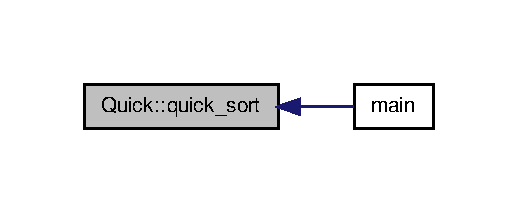
\includegraphics[width=248pt]{class_quick_a9104bc671992e64990dedf60c0dd6993_icgraph}
\end{center}
\end{figure}


\hypertarget{class_quick_abca7e1fcc40e88d337d81aeac1d98184}{\index{\-Quick@{\-Quick}!sprawdz\-\_\-porzadek@{sprawdz\-\_\-porzadek}}
\index{sprawdz\-\_\-porzadek@{sprawdz\-\_\-porzadek}!Quick@{\-Quick}}
\subsubsection[{sprawdz\-\_\-porzadek}]{\setlength{\rightskip}{0pt plus 5cm}template$<$typename T $>$ bool {\bf \-Quick\-::sprawdz\-\_\-porzadek} (
\begin{DoxyParamCaption}
\item[{\-T $\ast$$\ast$}]{tab, }
\item[{int}]{rozmiar}
\end{DoxyParamCaption}
)}}\label{class_quick_abca7e1fcc40e88d337d81aeac1d98184}


\-Oto graf wywoływań tej funkcji\-:\nopagebreak
\begin{figure}[H]
\begin{center}
\leavevmode
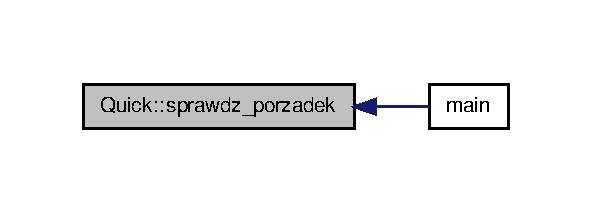
\includegraphics[width=284pt]{class_quick_abca7e1fcc40e88d337d81aeac1d98184_icgraph}
\end{center}
\end{figure}


\hypertarget{class_quick_aad4bc8adc3139667f2edaa1e46993b6e}{\index{\-Quick@{\-Quick}!wypelnij@{wypelnij}}
\index{wypelnij@{wypelnij}!Quick@{\-Quick}}
\subsubsection[{wypelnij}]{\setlength{\rightskip}{0pt plus 5cm}template$<$typename T $>$ void {\bf \-Quick\-::wypelnij} (
\begin{DoxyParamCaption}
\item[{\-T $\ast$$\ast$}]{tab, }
\item[{int}]{rozmiar, }
\item[{int}]{procent\-\_\-posortowanych}
\end{DoxyParamCaption}
)}}\label{class_quick_aad4bc8adc3139667f2edaa1e46993b6e}
\hypertarget{class_quick_a6029457895c0ec57c016c57be5bac0f1}{\index{\-Quick@{\-Quick}!wypelnij\-\_\-odwrotnie@{wypelnij\-\_\-odwrotnie}}
\index{wypelnij\-\_\-odwrotnie@{wypelnij\-\_\-odwrotnie}!Quick@{\-Quick}}
\subsubsection[{wypelnij\-\_\-odwrotnie}]{\setlength{\rightskip}{0pt plus 5cm}template$<$typename T $>$ void {\bf \-Quick\-::wypelnij\-\_\-odwrotnie} (
\begin{DoxyParamCaption}
\item[{\-T $\ast$$\ast$}]{tab, }
\item[{int}]{rozmiar}
\end{DoxyParamCaption}
)}}\label{class_quick_a6029457895c0ec57c016c57be5bac0f1}


\-Oto graf wywoływań tej funkcji\-:\nopagebreak
\begin{figure}[H]
\begin{center}
\leavevmode
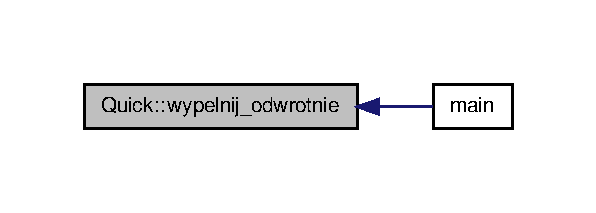
\includegraphics[width=286pt]{class_quick_a6029457895c0ec57c016c57be5bac0f1_icgraph}
\end{center}
\end{figure}


\hypertarget{class_quick_a407bd1912126105f6116393e7676fc05}{\index{\-Quick@{\-Quick}!wyswietl@{wyswietl}}
\index{wyswietl@{wyswietl}!Quick@{\-Quick}}
\subsubsection[{wyswietl}]{\setlength{\rightskip}{0pt plus 5cm}template$<$typename T $>$ void {\bf \-Quick\-::wyswietl} (
\begin{DoxyParamCaption}
\item[{\-T $\ast$}]{\-Poczatek, }
\item[{\-T $\ast$}]{\-Koniec}
\end{DoxyParamCaption}
)}}\label{class_quick_a407bd1912126105f6116393e7676fc05}
\hypertarget{class_quick_ab05c6bf9a4fe9d0ed6f83ee02c401ab9}{\index{\-Quick@{\-Quick}!wyswietl@{wyswietl}}
\index{wyswietl@{wyswietl}!Quick@{\-Quick}}
\subsubsection[{wyswietl}]{\setlength{\rightskip}{0pt plus 5cm}template$<$typename T $>$ void {\bf \-Quick\-::wyswietl} (
\begin{DoxyParamCaption}
\item[{\-T $\ast$$\ast$}]{tab, }
\item[{int}]{rozmiar}
\end{DoxyParamCaption}
)}}\label{class_quick_ab05c6bf9a4fe9d0ed6f83ee02c401ab9}


\-Dokumentacja dla tej klasy została wygenerowana z pliku\-:\begin{DoxyCompactItemize}
\item 
\hyperlink{quick_8hpp}{quick.\-hpp}\end{DoxyCompactItemize}

\hypertarget{class_tablica}{\section{\-Dokumentacja szablonu klasy \-Tablica$<$ \-K, \-W $>$}
\label{class_tablica}\index{\-Tablica$<$ K, W $>$@{\-Tablica$<$ K, W $>$}}
}


{\ttfamily \#include $<$\-Tablica.\-h$>$}

\subsection*{\-Metody publiczne}
\begin{DoxyCompactItemize}
\item 
\hyperlink{class_tablica_ae1408ffc077347605b61ea0899ddebed}{\-Tablica} (int \hyperlink{class_tablica_a40b3c86ceb2ec860b9d19ce0e866b406}{rozmiar})
\item 
\hyperlink{class_tablica_aabb6e01e32fd2d32ddcfba2c10b9ec5e}{$\sim$\-Tablica} ()
\item 
void \hyperlink{class_tablica_aebb17d3366e37c8b4852df08eae2a1de}{dodaj} (\hyperlink{class_para}{\-Para}$<$ \-K, \-W $>$ \&para)
\item 
void \hyperlink{class_tablica_a061a219dd25c6696940f40226d99a99d}{usun} (\-K klucz)
\item 
\-W \hyperlink{class_tablica_a6de46e3062f16d78c4cb2cf18c9b0de1}{pobierz\-Wartosc} (\-K klucz)
\item 
bool \hyperlink{class_tablica_a19d8da0353d73517375cf6b2984f9d5c}{czypusta} ()
\item 
int \hyperlink{class_tablica_aabc40f316cf398a07e3035b1c4adc256}{size} ()
\item 
\-W \& \hyperlink{class_tablica_a7f5a2d2ebe594ec98dd38dfbbb83497d}{operator\mbox{[}$\,$\mbox{]}} (\-K klucz)
\end{DoxyCompactItemize}
\subsection*{\-Metody prywatne}
\begin{DoxyCompactItemize}
\item 
int \hyperlink{class_tablica_a8fd66d75553eb44aa043f917fd9317dc}{haszstring} (\-K key)
\end{DoxyCompactItemize}
\subsection*{\-Atrybuty prywatne}
\begin{DoxyCompactItemize}
\item 
\hyperlink{class_para}{\-Para}$<$ \-K, \-W $>$ $\ast$$\ast$ \hyperlink{class_tablica_a0d6b03ac0a2b996d4096038ef9315e9a}{tablica}
\item 
int \hyperlink{class_tablica_a603b571fcc0d29b757bfd5fe27d0fadc}{liczba\-Elementow}
\item 
int \hyperlink{class_tablica_a40b3c86ceb2ec860b9d19ce0e866b406}{rozmiar}
\end{DoxyCompactItemize}


\subsection{\-Opis szczegółowy}
\subsubsection*{template$<$typename \-K, typename \-W$>$class Tablica$<$ K, W $>$}

\-Modeluje pojecie tablicy z haszowaniem. \-Klasa modeluje pojecie tablicy z haszowaniem. \-Jej atrybutami sa pola\-: klucz i wartosc. 

\subsection{\-Dokumentacja konstruktora i destruktora}
\hypertarget{class_tablica_ae1408ffc077347605b61ea0899ddebed}{\index{\-Tablica@{\-Tablica}!\-Tablica@{\-Tablica}}
\index{\-Tablica@{\-Tablica}!Tablica@{\-Tablica}}
\subsubsection[{\-Tablica}]{\setlength{\rightskip}{0pt plus 5cm}template$<$typename K , typename W $>$ {\bf \-Tablica}$<$ \-K, \-W $>$\-::{\bf \-Tablica} (
\begin{DoxyParamCaption}
\item[{int}]{rozmiar}
\end{DoxyParamCaption}
)}}\label{class_tablica_ae1408ffc077347605b61ea0899ddebed}


\-Konstruktor klasy \hyperlink{class_tablica}{\-Tablica}. \-Jego argumentem jest maksymalny rozmiar tablicy. 

\hypertarget{class_tablica_aabb6e01e32fd2d32ddcfba2c10b9ec5e}{\index{\-Tablica@{\-Tablica}!$\sim$\-Tablica@{$\sim$\-Tablica}}
\index{$\sim$\-Tablica@{$\sim$\-Tablica}!Tablica@{\-Tablica}}
\subsubsection[{$\sim$\-Tablica}]{\setlength{\rightskip}{0pt plus 5cm}template$<$typename K , typename W $>$ {\bf \-Tablica}$<$ \-K, \-W $>$\-::$\sim${\bf \-Tablica} (
\begin{DoxyParamCaption}
{}
\end{DoxyParamCaption}
)}}\label{class_tablica_aabb6e01e32fd2d32ddcfba2c10b9ec5e}


\-Destruktor klasy \hyperlink{class_tablica}{\-Tablica}. \-Czysci pamiec. 



\subsection{\-Dokumentacja funkcji składowych}
\hypertarget{class_tablica_a19d8da0353d73517375cf6b2984f9d5c}{\index{\-Tablica@{\-Tablica}!czypusta@{czypusta}}
\index{czypusta@{czypusta}!Tablica@{\-Tablica}}
\subsubsection[{czypusta}]{\setlength{\rightskip}{0pt plus 5cm}template$<$typename \-K, typename \-W$>$ bool {\bf \-Tablica}$<$ \-K, \-W $>$\-::{\bf czypusta} (
\begin{DoxyParamCaption}
{}
\end{DoxyParamCaption}
)\hspace{0.3cm}{\ttfamily  \mbox{[}inline\mbox{]}}}}\label{class_tablica_a19d8da0353d73517375cf6b2984f9d5c}


\-Sprawdza zapelnienie tablicy. 

\begin{DoxyReturn}{\-Zwraca}
zwraca prawde, gdy tablica jest pusta 
\end{DoxyReturn}
\hypertarget{class_tablica_aebb17d3366e37c8b4852df08eae2a1de}{\index{\-Tablica@{\-Tablica}!dodaj@{dodaj}}
\index{dodaj@{dodaj}!Tablica@{\-Tablica}}
\subsubsection[{dodaj}]{\setlength{\rightskip}{0pt plus 5cm}template$<$typename K , typename W $>$ void {\bf \-Tablica}$<$ \-K, \-W $>$\-::{\bf dodaj} (
\begin{DoxyParamCaption}
\item[{{\bf \-Para}$<$ \-K, \-W $>$ \&}]{para}
\end{DoxyParamCaption}
)}}\label{class_tablica_aebb17d3366e37c8b4852df08eae2a1de}


\-Funkcja dodaj. \-Dodaje krotke do tablicy. 



\-Oto graf wywołań dla tej funkcji\-:\nopagebreak
\begin{figure}[H]
\begin{center}
\leavevmode
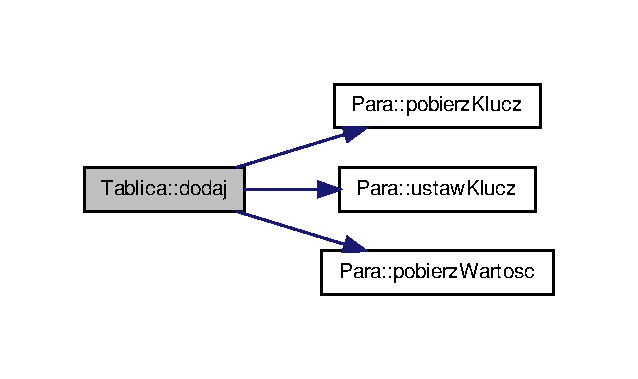
\includegraphics[width=306pt]{class_tablica_aebb17d3366e37c8b4852df08eae2a1de_cgraph}
\end{center}
\end{figure}




\-Oto graf wywoływań tej funkcji\-:\nopagebreak
\begin{figure}[H]
\begin{center}
\leavevmode
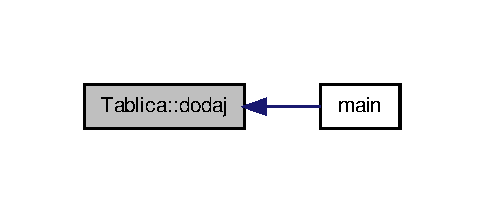
\includegraphics[width=232pt]{class_tablica_aebb17d3366e37c8b4852df08eae2a1de_icgraph}
\end{center}
\end{figure}


\hypertarget{class_tablica_a8fd66d75553eb44aa043f917fd9317dc}{\index{\-Tablica@{\-Tablica}!haszstring@{haszstring}}
\index{haszstring@{haszstring}!Tablica@{\-Tablica}}
\subsubsection[{haszstring}]{\setlength{\rightskip}{0pt plus 5cm}template$<$typename K , typename W $>$ int {\bf \-Tablica}$<$ \-K, \-W $>$\-::{\bf haszstring} (
\begin{DoxyParamCaption}
\item[{\-K}]{key}
\end{DoxyParamCaption}
)\hspace{0.3cm}{\ttfamily  \mbox{[}private\mbox{]}}}}\label{class_tablica_a8fd66d75553eb44aa043f917fd9317dc}


\-Funkcja haszujaca dla obiektow typu string. 

\hypertarget{class_tablica_a7f5a2d2ebe594ec98dd38dfbbb83497d}{\index{\-Tablica@{\-Tablica}!operator\mbox{[}$\,$\mbox{]}@{operator[]}}
\index{operator\mbox{[}$\,$\mbox{]}@{operator[]}!Tablica@{\-Tablica}}
\subsubsection[{operator[]}]{\setlength{\rightskip}{0pt plus 5cm}template$<$typename K , typename W $>$ \-W \& {\bf \-Tablica}$<$ \-K, \-W $>$\-::operator\mbox{[}$\,$\mbox{]} (
\begin{DoxyParamCaption}
\item[{\-K}]{klucz}
\end{DoxyParamCaption}
)}}\label{class_tablica_a7f5a2d2ebe594ec98dd38dfbbb83497d}


\-Przeciazenie operatora indeksujacego. 

\begin{DoxyReturn}{\-Zwraca}
\-Zwraca wartosc. 
\end{DoxyReturn}


\-Oto graf wywołań dla tej funkcji\-:\nopagebreak
\begin{figure}[H]
\begin{center}
\leavevmode
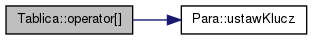
\includegraphics[width=306pt]{class_tablica_a7f5a2d2ebe594ec98dd38dfbbb83497d_cgraph}
\end{center}
\end{figure}


\hypertarget{class_tablica_a6de46e3062f16d78c4cb2cf18c9b0de1}{\index{\-Tablica@{\-Tablica}!pobierz\-Wartosc@{pobierz\-Wartosc}}
\index{pobierz\-Wartosc@{pobierz\-Wartosc}!Tablica@{\-Tablica}}
\subsubsection[{pobierz\-Wartosc}]{\setlength{\rightskip}{0pt plus 5cm}template$<$typename K , typename W $>$ \-W {\bf \-Tablica}$<$ \-K, \-W $>$\-::{\bf pobierz\-Wartosc} (
\begin{DoxyParamCaption}
\item[{\-K}]{klucz}
\end{DoxyParamCaption}
)}}\label{class_tablica_a6de46e3062f16d78c4cb2cf18c9b0de1}


\-Funkcja pobierz\-Wartosc. 

\begin{DoxyReturn}{\-Zwraca}
\-Zwraca wartosc przypisana do danego klucza. 
\end{DoxyReturn}


\-Oto graf wywoływań tej funkcji\-:\nopagebreak
\begin{figure}[H]
\begin{center}
\leavevmode
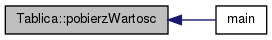
\includegraphics[width=276pt]{class_tablica_a6de46e3062f16d78c4cb2cf18c9b0de1_icgraph}
\end{center}
\end{figure}


\hypertarget{class_tablica_aabc40f316cf398a07e3035b1c4adc256}{\index{\-Tablica@{\-Tablica}!size@{size}}
\index{size@{size}!Tablica@{\-Tablica}}
\subsubsection[{size}]{\setlength{\rightskip}{0pt plus 5cm}template$<$typename \-K, typename \-W$>$ int {\bf \-Tablica}$<$ \-K, \-W $>$\-::{\bf size} (
\begin{DoxyParamCaption}
{}
\end{DoxyParamCaption}
)\hspace{0.3cm}{\ttfamily  \mbox{[}inline\mbox{]}}}}\label{class_tablica_aabc40f316cf398a07e3035b1c4adc256}


\-Podaje liczbe elementow w tablicy. 

\begin{DoxyReturn}{\-Zwraca}
zwraca liczbe elementow w tablicy. 
\end{DoxyReturn}
\hypertarget{class_tablica_a061a219dd25c6696940f40226d99a99d}{\index{\-Tablica@{\-Tablica}!usun@{usun}}
\index{usun@{usun}!Tablica@{\-Tablica}}
\subsubsection[{usun}]{\setlength{\rightskip}{0pt plus 5cm}template$<$typename K , typename W $>$ void {\bf \-Tablica}$<$ \-K, \-W $>$\-::{\bf usun} (
\begin{DoxyParamCaption}
\item[{\-K}]{klucz}
\end{DoxyParamCaption}
)}}\label{class_tablica_a061a219dd25c6696940f40226d99a99d}


\-Funkcja usun. \-Usuwa krotke o podanym kluczu. 



\-Oto graf wywoływań tej funkcji\-:\nopagebreak
\begin{figure}[H]
\begin{center}
\leavevmode
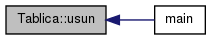
\includegraphics[width=230pt]{class_tablica_a061a219dd25c6696940f40226d99a99d_icgraph}
\end{center}
\end{figure}




\subsection{\-Dokumentacja atrybutów składowych}
\hypertarget{class_tablica_a603b571fcc0d29b757bfd5fe27d0fadc}{\index{\-Tablica@{\-Tablica}!liczba\-Elementow@{liczba\-Elementow}}
\index{liczba\-Elementow@{liczba\-Elementow}!Tablica@{\-Tablica}}
\subsubsection[{liczba\-Elementow}]{\setlength{\rightskip}{0pt plus 5cm}template$<$typename \-K, typename \-W$>$ int {\bf \-Tablica}$<$ \-K, \-W $>$\-::{\bf liczba\-Elementow}\hspace{0.3cm}{\ttfamily  \mbox{[}private\mbox{]}}}}\label{class_tablica_a603b571fcc0d29b757bfd5fe27d0fadc}


\-Obecna liczba elementow w tablicy. 

\hypertarget{class_tablica_a40b3c86ceb2ec860b9d19ce0e866b406}{\index{\-Tablica@{\-Tablica}!rozmiar@{rozmiar}}
\index{rozmiar@{rozmiar}!Tablica@{\-Tablica}}
\subsubsection[{rozmiar}]{\setlength{\rightskip}{0pt plus 5cm}template$<$typename \-K, typename \-W$>$ int {\bf \-Tablica}$<$ \-K, \-W $>$\-::{\bf rozmiar}\hspace{0.3cm}{\ttfamily  \mbox{[}private\mbox{]}}}}\label{class_tablica_a40b3c86ceb2ec860b9d19ce0e866b406}


\-Maksymalna liczba elementow w tablicy. 

\hypertarget{class_tablica_a0d6b03ac0a2b996d4096038ef9315e9a}{\index{\-Tablica@{\-Tablica}!tablica@{tablica}}
\index{tablica@{tablica}!Tablica@{\-Tablica}}
\subsubsection[{tablica}]{\setlength{\rightskip}{0pt plus 5cm}template$<$typename \-K, typename \-W$>$ {\bf \-Para}$<$\-K,\-W$>$$\ast$$\ast$ {\bf \-Tablica}$<$ \-K, \-W $>$\-::{\bf tablica}\hspace{0.3cm}{\ttfamily  \mbox{[}private\mbox{]}}}}\label{class_tablica_a0d6b03ac0a2b996d4096038ef9315e9a}


\hyperlink{class_tablica}{\-Tablica} par. 



\-Dokumentacja dla tej klasy została wygenerowana z pliku\-:\begin{DoxyCompactItemize}
\item 
\hyperlink{_tablica_8h}{\-Tablica.\-h}\end{DoxyCompactItemize}

\chapter{\-Dokumentacja plików}
\hypertarget{dzialania_8cpp}{\section{\-Dokumentacja pliku dzialania.\-cpp}
\label{dzialania_8cpp}\index{dzialania.\-cpp@{dzialania.\-cpp}}
}
{\ttfamily \#include $<$iostream$>$}\*
{\ttfamily \#include $<$fstream$>$}\*
{\ttfamily \#include \char`\"{}../inc/dzialania.\-hpp\char`\"{}}\*
{\ttfamily \#include $<$ctime$>$}\*
\-Wykres zależności załączania dla dzialania.\-cpp\-:\nopagebreak
\begin{figure}[H]
\begin{center}
\leavevmode
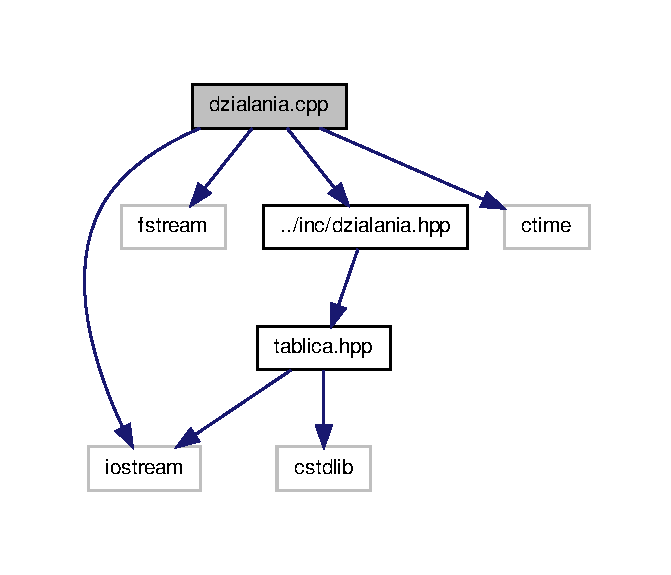
\includegraphics[width=322pt]{dzialania_8cpp__incl}
\end{center}
\end{figure}
\subsection*{\-Funkcje}
\begin{DoxyCompactItemize}
\item 
void \hyperlink{dzialania_8cpp_ac07863d69ae41a4e395b31f73b35fbcd}{foo} ()
\end{DoxyCompactItemize}


\subsection{\-Dokumentacja funkcji}
\hypertarget{dzialania_8cpp_ac07863d69ae41a4e395b31f73b35fbcd}{\index{dzialania.\-cpp@{dzialania.\-cpp}!foo@{foo}}
\index{foo@{foo}!dzialania.cpp@{dzialania.\-cpp}}
\subsubsection[{foo}]{\setlength{\rightskip}{0pt plus 5cm}void {\bf foo} (
\begin{DoxyParamCaption}
{}
\end{DoxyParamCaption}
)}}\label{dzialania_8cpp_ac07863d69ae41a4e395b31f73b35fbcd}

\hypertarget{dzialania_8hpp}{\section{\-Dokumentacja pliku dzialania.\-hpp}
\label{dzialania_8hpp}\index{dzialania.\-hpp@{dzialania.\-hpp}}
}
{\ttfamily \#include \char`\"{}tablica.\-hpp\char`\"{}}\*
\-Wykres zależności załączania dla dzialania.\-hpp\-:\nopagebreak
\begin{figure}[H]
\begin{center}
\leavevmode
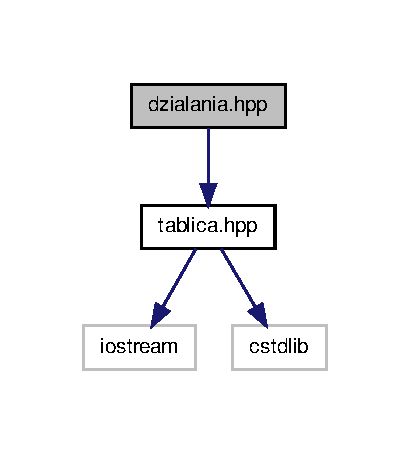
\includegraphics[width=196pt]{dzialania_8hpp__incl}
\end{center}
\end{figure}
\-Ten wykres pokazuje, które pliki bezpośrednio lub pośrednio załączają ten plik\-:\nopagebreak
\begin{figure}[H]
\begin{center}
\leavevmode
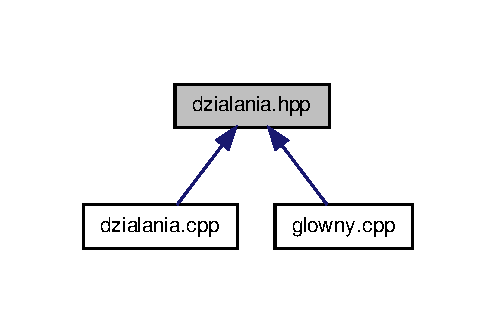
\includegraphics[width=238pt]{dzialania_8hpp__dep__incl}
\end{center}
\end{figure}
\subsection*{\-Komponenty}
\begin{DoxyCompactItemize}
\item 
class \hyperlink{class_dzialania}{\-Dzialania}
\begin{DoxyCompactList}\small\item\em \-Deklaracja klasy \hyperlink{class_dzialania}{\-Dzialania}. \end{DoxyCompactList}\end{DoxyCompactItemize}
\subsection*{\-Funkcje}
\begin{DoxyCompactItemize}
\item 
void \hyperlink{dzialania_8hpp_ac07863d69ae41a4e395b31f73b35fbcd}{foo} ()
\end{DoxyCompactItemize}


\subsection{\-Dokumentacja funkcji}
\hypertarget{dzialania_8hpp_ac07863d69ae41a4e395b31f73b35fbcd}{\index{dzialania.\-hpp@{dzialania.\-hpp}!foo@{foo}}
\index{foo@{foo}!dzialania.hpp@{dzialania.\-hpp}}
\subsubsection[{foo}]{\setlength{\rightskip}{0pt plus 5cm}void {\bf foo} (
\begin{DoxyParamCaption}
{}
\end{DoxyParamCaption}
)}}\label{dzialania_8hpp_ac07863d69ae41a4e395b31f73b35fbcd}

\hypertarget{glowny_8cpp}{\section{\-Dokumentacja pliku glowny.\-cpp}
\label{glowny_8cpp}\index{glowny.\-cpp@{glowny.\-cpp}}
}
{\ttfamily \#include $<$iostream$>$}\*
{\ttfamily \#include $<$string$>$}\*
{\ttfamily \#include $<$cstdlib$>$}\*
{\ttfamily \#include $<$fstream$>$}\*
{\ttfamily \#include $<$ctime$>$}\*
{\ttfamily \#include \char`\"{}../inc/quick.\-hpp\char`\"{}}\*
{\ttfamily \#include \char`\"{}../inc/tablica.\-hpp\char`\"{}}\*
{\ttfamily \#include \char`\"{}../inc/dzialania.\-hpp\char`\"{}}\*
{\ttfamily \#include \char`\"{}../inc/merge.\-hpp\char`\"{}}\*
\-Wykres zależności załączania dla glowny.\-cpp\-:\nopagebreak
\begin{figure}[H]
\begin{center}
\leavevmode
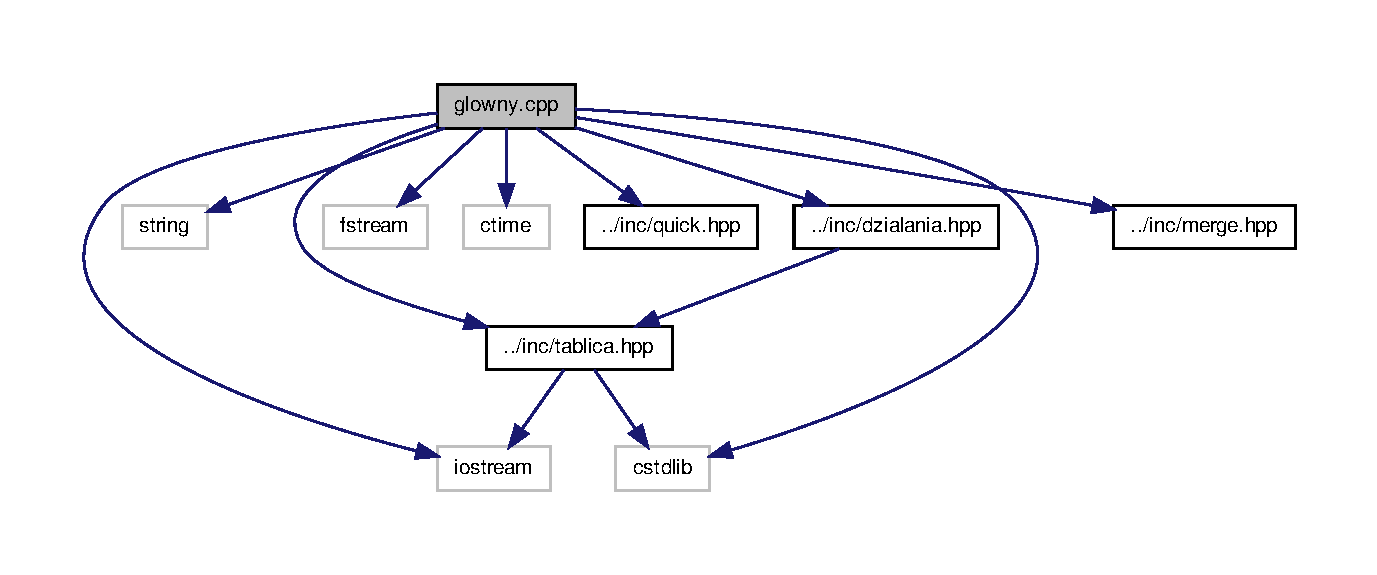
\includegraphics[width=350pt]{glowny_8cpp__incl}
\end{center}
\end{figure}
\subsection*{\-Definicje}
\begin{DoxyCompactItemize}
\item 
\#define \hyperlink{glowny_8cpp_aa50aa866c5823769bb02e986d29a0589}{\-R\-O\-Z\-M\-I\-A\-R}~20
\end{DoxyCompactItemize}
\subsection*{\-Funkcje}
\begin{DoxyCompactItemize}
\item 
int \hyperlink{glowny_8cpp_a3c04138a5bfe5d72780bb7e82a18e627}{main} (int argc, char $\ast$$\ast$argv)
\end{DoxyCompactItemize}


\subsection{\-Dokumentacja definicji}
\hypertarget{glowny_8cpp_aa50aa866c5823769bb02e986d29a0589}{\index{glowny.\-cpp@{glowny.\-cpp}!\-R\-O\-Z\-M\-I\-A\-R@{\-R\-O\-Z\-M\-I\-A\-R}}
\index{\-R\-O\-Z\-M\-I\-A\-R@{\-R\-O\-Z\-M\-I\-A\-R}!glowny.cpp@{glowny.\-cpp}}
\subsubsection[{\-R\-O\-Z\-M\-I\-A\-R}]{\setlength{\rightskip}{0pt plus 5cm}\#define {\bf \-R\-O\-Z\-M\-I\-A\-R}~20}}\label{glowny_8cpp_aa50aa866c5823769bb02e986d29a0589}


\subsection{\-Dokumentacja funkcji}
\hypertarget{glowny_8cpp_a3c04138a5bfe5d72780bb7e82a18e627}{\index{glowny.\-cpp@{glowny.\-cpp}!main@{main}}
\index{main@{main}!glowny.cpp@{glowny.\-cpp}}
\subsubsection[{main}]{\setlength{\rightskip}{0pt plus 5cm}int {\bf main} (
\begin{DoxyParamCaption}
\item[{int}]{argc, }
\item[{char $\ast$$\ast$}]{argv}
\end{DoxyParamCaption}
)}}\label{glowny_8cpp_a3c04138a5bfe5d72780bb7e82a18e627}


\-Glowna funkcja programu. 

\-Wyświetla wynik pomiarowy tablicy. 

\-Oto graf wywołań dla tej funkcji\-:\nopagebreak
\begin{figure}[H]
\begin{center}
\leavevmode
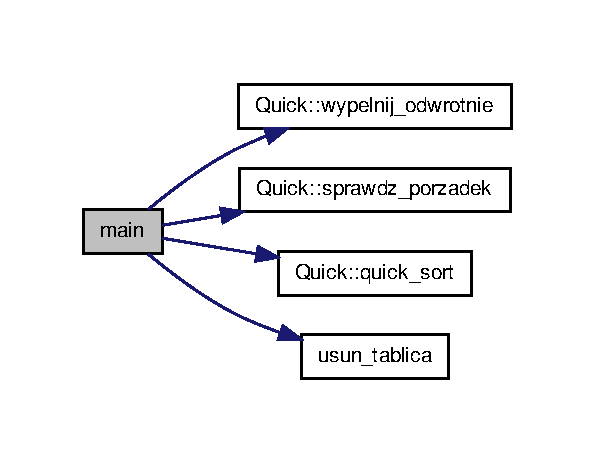
\includegraphics[width=286pt]{glowny_8cpp_a3c04138a5bfe5d72780bb7e82a18e627_cgraph}
\end{center}
\end{figure}



\hypertarget{merge_8cpp}{\section{\-Dokumentacja pliku merge.\-cpp}
\label{merge_8cpp}\index{merge.\-cpp@{merge.\-cpp}}
}
{\ttfamily \#include $<$iostream$>$}\*
{\ttfamily \#include $<$cstdlib$>$}\*
{\ttfamily \#include $<$ctime$>$}\*
\-Wykres zależności załączania dla merge.\-cpp\-:\nopagebreak
\begin{figure}[H]
\begin{center}
\leavevmode
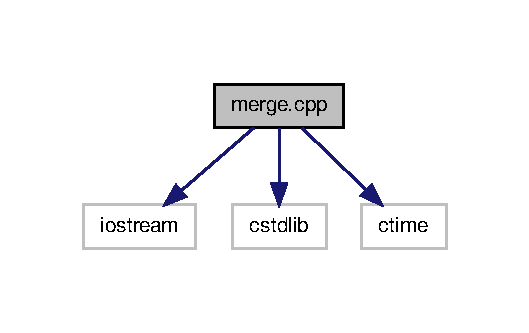
\includegraphics[width=254pt]{merge_8cpp__incl}
\end{center}
\end{figure}

\hypertarget{merge_8hpp}{\section{\-Dokumentacja pliku merge.\-hpp}
\label{merge_8hpp}\index{merge.\-hpp@{merge.\-hpp}}
}


\-Plik zawiera definicje funkcji sortowania merge.  


\-Ten wykres pokazuje, które pliki bezpośrednio lub pośrednio załączają ten plik\-:\nopagebreak
\begin{figure}[H]
\begin{center}
\leavevmode
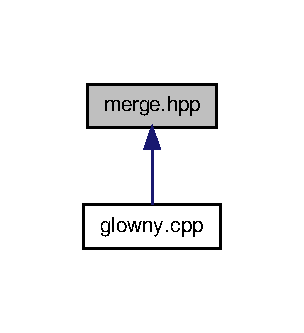
\includegraphics[width=184pt]{merge_8hpp__dep__incl}
\end{center}
\end{figure}
\subsection*{\-Komponenty}
\begin{DoxyCompactItemize}
\item 
class \hyperlink{class_merge}{\-Merge}
\begin{DoxyCompactList}\small\item\em \-Modeluje pojecie \hyperlink{class_merge}{\-Merge}. \-Szablon funkcji sortowania przez scalanie. \end{DoxyCompactList}\end{DoxyCompactItemize}


\subsection{\-Opis szczegółowy}


\-Definicja w pliku \hyperlink{merge_8hpp_source}{merge.\-hpp}.


\hypertarget{quick_8cpp}{\section{\-Dokumentacja pliku quick.\-cpp}
\label{quick_8cpp}\index{quick.\-cpp@{quick.\-cpp}}
}

\hypertarget{quick_8hpp}{\section{\-Dokumentacja pliku quick.\-hpp}
\label{quick_8hpp}\index{quick.\-hpp@{quick.\-hpp}}
}
\-Ten wykres pokazuje, które pliki bezpośrednio lub pośrednio załączają ten plik\-:\nopagebreak
\begin{figure}[H]
\begin{center}
\leavevmode
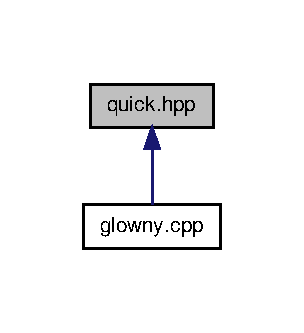
\includegraphics[width=146pt]{quick_8hpp__dep__incl}
\end{center}
\end{figure}
\subsection*{\-Komponenty}
\begin{DoxyCompactItemize}
\item 
class \hyperlink{class_quick}{\-Quick}
\end{DoxyCompactItemize}
\subsection*{\-Funkcje}
\begin{DoxyCompactItemize}
\item 
void \hyperlink{quick_8hpp_acd68a470bbe53460d819b0cea1d7a8e1}{usun\-\_\-tablica} (int $\ast$$\ast$tab)
\end{DoxyCompactItemize}


\subsection{\-Dokumentacja funkcji}
\hypertarget{quick_8hpp_acd68a470bbe53460d819b0cea1d7a8e1}{\index{quick.\-hpp@{quick.\-hpp}!usun\-\_\-tablica@{usun\-\_\-tablica}}
\index{usun\-\_\-tablica@{usun\-\_\-tablica}!quick.hpp@{quick.\-hpp}}
\subsubsection[{usun\-\_\-tablica}]{\setlength{\rightskip}{0pt plus 5cm}void {\bf usun\-\_\-tablica} (
\begin{DoxyParamCaption}
\item[{int $\ast$$\ast$}]{tab}
\end{DoxyParamCaption}
)}}\label{quick_8hpp_acd68a470bbe53460d819b0cea1d7a8e1}


\-Oto graf wywoływań tej funkcji\-:\nopagebreak
\begin{figure}[H]
\begin{center}
\leavevmode
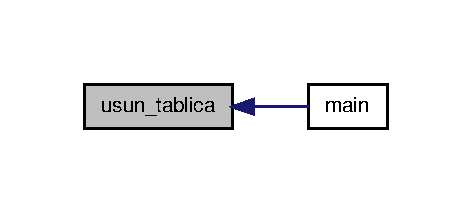
\includegraphics[width=226pt]{quick_8hpp_acd68a470bbe53460d819b0cea1d7a8e1_icgraph}
\end{center}
\end{figure}



\hypertarget{tablica_8cpp}{\section{\-Dokumentacja pliku tablica.\-cpp}
\label{tablica_8cpp}\index{tablica.\-cpp@{tablica.\-cpp}}
}
{\ttfamily \#include \char`\"{}../inc/tablica.\-hpp\char`\"{}}\*
{\ttfamily \#include $<$iostream$>$}\*
\-Wykres zależności załączania dla tablica.\-cpp\-:\nopagebreak
\begin{figure}[H]
\begin{center}
\leavevmode
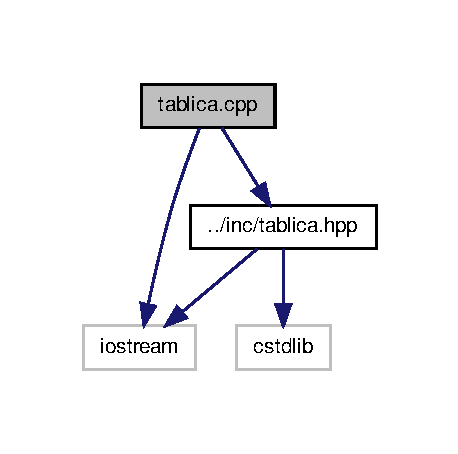
\includegraphics[width=220pt]{tablica_8cpp__incl}
\end{center}
\end{figure}
\subsection*{\-Funkcje}
\begin{DoxyCompactItemize}
\item 
void \hyperlink{tablica_8cpp_ac0a954582addc00e3370863ebbd82734}{foo22} ()
\end{DoxyCompactItemize}


\subsection{\-Dokumentacja funkcji}
\hypertarget{tablica_8cpp_ac0a954582addc00e3370863ebbd82734}{\index{tablica.\-cpp@{tablica.\-cpp}!foo22@{foo22}}
\index{foo22@{foo22}!tablica.cpp@{tablica.\-cpp}}
\subsubsection[{foo22}]{\setlength{\rightskip}{0pt plus 5cm}void {\bf foo22} (
\begin{DoxyParamCaption}
{}
\end{DoxyParamCaption}
)}}\label{tablica_8cpp_ac0a954582addc00e3370863ebbd82734}

\hypertarget{tablica_8hpp}{\section{\-Dokumentacja pliku tablica.\-hpp}
\label{tablica_8hpp}\index{tablica.\-hpp@{tablica.\-hpp}}
}
{\ttfamily \#include $<$iostream$>$}\*
{\ttfamily \#include $<$cstdlib$>$}\*
\-Wykres zależności załączania dla tablica.\-hpp\-:\nopagebreak
\begin{figure}[H]
\begin{center}
\leavevmode
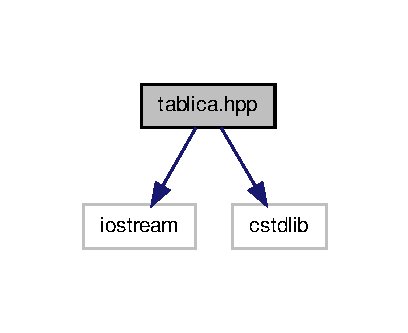
\includegraphics[width=196pt]{tablica_8hpp__incl}
\end{center}
\end{figure}
\-Ten wykres pokazuje, które pliki bezpośrednio lub pośrednio załączają ten plik\-:\nopagebreak
\begin{figure}[H]
\begin{center}
\leavevmode
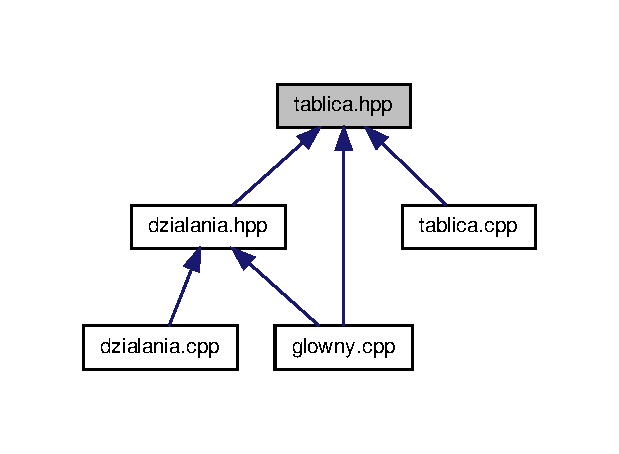
\includegraphics[width=297pt]{tablica_8hpp__dep__incl}
\end{center}
\end{figure}
\subsection*{\-Komponenty}
\begin{DoxyCompactItemize}
\item 
class \hyperlink{class_tablica}{\-Tablica$<$ Typ $>$}
\begin{DoxyCompactList}\small\item\em \-Klasa reprezentująca tablicę \end{DoxyCompactList}\end{DoxyCompactItemize}
\subsection*{\-Funkcje}
\begin{DoxyCompactItemize}
\item 
void \hyperlink{tablica_8hpp_ac0a954582addc00e3370863ebbd82734}{foo22} ()
\end{DoxyCompactItemize}


\subsection{\-Dokumentacja funkcji}
\hypertarget{tablica_8hpp_ac0a954582addc00e3370863ebbd82734}{\index{tablica.\-hpp@{tablica.\-hpp}!foo22@{foo22}}
\index{foo22@{foo22}!tablica.hpp@{tablica.\-hpp}}
\subsubsection[{foo22}]{\setlength{\rightskip}{0pt plus 5cm}void {\bf foo22} (
\begin{DoxyParamCaption}
{}
\end{DoxyParamCaption}
)}}\label{tablica_8hpp_ac0a954582addc00e3370863ebbd82734}

\printindex
\end{document}
